	\documentclass[a4paper]{article}
	
	\usepackage[portuguese]{babel}
	\usepackage[utf8]{inputenc}
	\usepackage{indentfirst}
	\usepackage{graphicx}
	\usepackage{verbatim}
	\usepackage{wrapfig, blindtext}
	\usepackage{listings}

	\begin{document}
	
	\setlength{\textwidth}{16cm}
	\setlength{\textheight}{22cm}
	
	\title{\Huge\textbf{Q!nto}\linebreak\linebreak\linebreak
	\Large\textbf{Relatório Intercalar}\linebreak\linebreak
	\linebreak\linebreak
	
\includegraphics[scale=0.1]{./res/feup-logo.png}\linebreak\linebreak
	\linebreak\linebreak
	\Large{Mestrado Integrado em Engenharia Informática e Computação} \linebreak\linebreak
	\Large{Programação em Lógica}\linebreak
		}
	

	\author{
	\textbf{Grupo Q!nto\_1:}\\
	João Miguel Fidalgo Esteves Nogueira - up201303882 \\
	Luís Miguel da Costa Oliveira - up201304515 \\
	\linebreak\linebreak \\
	 \\ Faculdade de Engenharia da Universidade do Porto \\ Rua Roberto Frias, s\/n, 4200-465 Porto, Portugal \linebreak\linebreak\linebreak
	\linebreak\linebreak\vspace{1cm}}
	
	\maketitle
	\thispagestyle{empty}
	
	\newpage
	
	\section{Descrição detalhada do Jogo}
	\subsection{História}
	
	“Q!nto” é um jogo de tabuleiro recente, criado no ano de 2014 no qual podem participar entre 2 e 4 jogadores. Foi criado por Gene Mackles e lançado pela PDG games
	
	Este jogo faz parte de uma coleção de três jogos chamada Triple Play que é uma coleção de jogos de tabuleiro.
	
	\begin{wrapfigure}{R}{0.4\textwidth}
	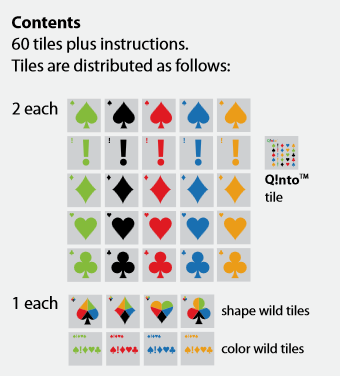
\includegraphics[width=0.4\textwidth]{./res/cards.png}
	\caption{\label{fig:Baralho}Baralho}
	\end{wrapfigure}
	
	\subsection{Conteúdo do Jogo}
	
	Estão incluídas no Jogo 60 cartas divididas como mostra a figura à direita.
	
	\subsection{Regras de Jogo}
	
	Existem três versões para jogar o Q!into, sendo elas o
	\textit{Classic},
	\textit{Plus} e
	\textit{Light}. Neste projeto usaremos apenas a versão Light que passamos a explicar a seguir:
	
	Inicialmente cada jogador retira uma carta do baralho para escolher quem começa a jogar. O jogador cuja carta tem o naipe mais alto começa, sendo que a hierarquia é a definida na imagem acima (de cima para baixo). O jogo começa dividindo igualmente o baralho pelos jogadores presentes.
	
	As cartas que cada jogador recebeu serão a pilha de cartas com que ele vai poder jogar. Estas ficarão viradas para baixo e cada jogador retira da pilha de cartas que lhe foi atribuída as primeiras 5. 
	
	\textbf{Noção base:} Uma linha são 2, 3, 4 ou 5 cartas numa linha ou coluna na qual as cartas têm a mesma côr ou cores diferentes e na qual as cartas têm a mesma forma ou formas diferentes. Uma linha com 5 cartas é um Q!nto.
	O primeiro jogador começa o jogo. A seguir joga o jogador à sua esquerda. Quando na vez de um jogador, este pode fazer uma de três coisas:
	
	\begin{enumerate}
	\item 		Adicionar 1, 2, 3, 4 ou 5 peças à grelha numa única linha reta e depois retirar do topo da sua pilha de cartas o número necesário para voltar a ficar com 5 na mão*.
	Se, numa das jogadas, o jogador completar um ou mais Q!ntos, este deve voltar a completar a sua mão* e deve jogar outra vez.
	\item		Trocar uma ou mais cartas da sua mão por wildcards já jogadas e/ou a carta Q!nto de forma a que as cartas trocadas continuem a funcionar naquela posição.
	\item		Passar a vez... e trocar algumas, todas ou nenhuma das susas cartas colocando-as no fundo da sua pilha e retirando do topo o número de cartas necessário para voltar a ficar com 5*.
	\end{enumerate}
	
	\small
	*ou menos, se não houver cartas suficientes para perfazer 5.
	\normalsize
	
	\bigskip
	
	O jogo termina quando houver 1 jogador que fica sem cartas, sendo este o vencedor.\newline
	
	\small
	\noindent
	Nota: Uma carta “wild” ou “Q!nto” pode representar cartas diferentes em diferentes direções. No caso de representar coisas diferentes e não ter na mão uma carta que também as consiga representar, então, essa carta é insubstituível.
	\normalsize
	
	%************************************************************************************************
	\section{Representação do estado do Jogo}

	O \textit{Q!nto}, embora não seja um jogo de tabuleiro, basea-se na posição relativa das cartas na mesa. Por esse motivo optámos por guardar a informação do jogo numa lista de listas. Esta lista de listas será representada no ecrã tal como um tabuleiro.
	
	\subsection{Código da estrutura de dados da mesa}
	
	\small
	\lstset{language=Prolog}
	\lstinputlisting{./res/createTable.pl}
	\normalsize
	O código acima é responsável por criar uma lista de listas que representam uma lista de linhas para guardar a informação do conteúdo da mesa. Como é suposto no início do jogo, a mesa é inicializada como vazia.\\
	
	\newpage
	
	\subsection{Código de representação do Ambiente de jogo}
	\small
	\lstset{language=Prolog}
	\lstinputlisting{./res/print.pl}
	\normalsize
	O Código acima é responsável por inicializar a mesa e imprimi-la no ecrã.
	
	No entanto, este não é todo o código responsável pela impressão da lista de listas. Os predicados em falta percorrem as linhas imprimindo cada elemento, tal como se certificam de que a formatação do texto é a mais correta possível por forma a garantir que o utilizador tem uma forma eficiente de perceber o estado atual do jogo.
	
	\begin{figure}[h!]
	\begin{center}
	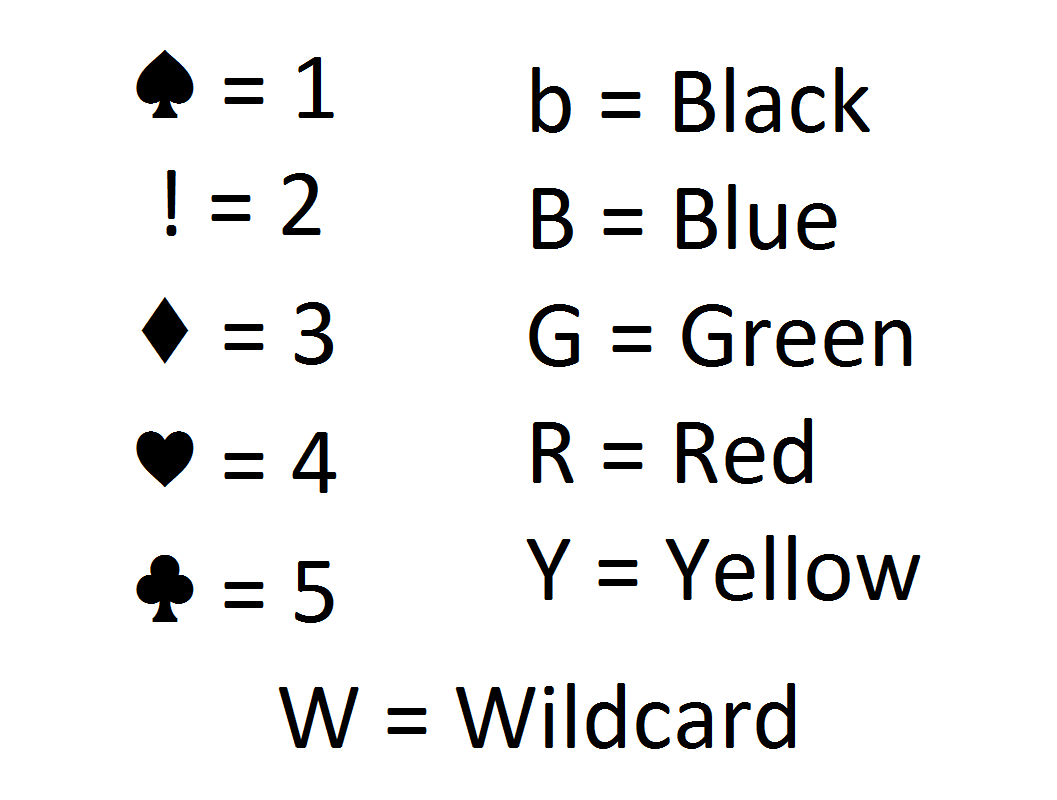
\includegraphics[scale=0.2]{./res/cardCode.png}
	\caption{Código das Cartas}
	\label{fig:example1}
	\end{center}
	\end{figure}
	
	\newpage
	\subsection{Exemplos de Ambientes de jogo}
	
	\begin{figure}[h!]
	\begin{center}
	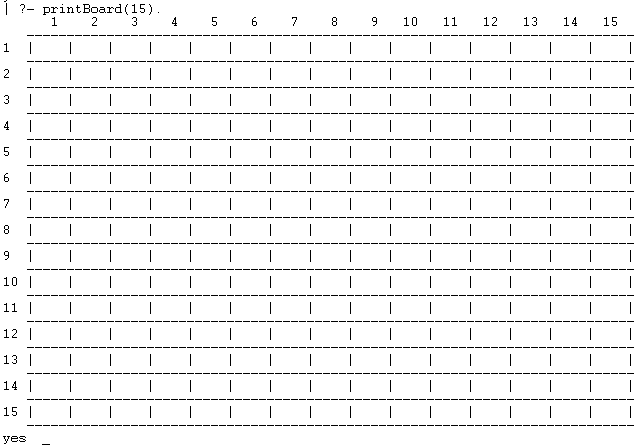
\includegraphics[scale=0.7]{./res/example_1.png}
	\caption{Exemplo de Ambiente Gráfico}
	\label{fig:example1}
	\end{center}
	\end{figure}
	
	\newpage
	
	Código de estados pré-definidos e respetiva apresentação.
	
	\footnotesize
	\lstset{language=Prolog}
	\lstinputlisting[tabsize=1]{./res/preset.pl}
	\normalsize
	
	\begin{figure}[h!]
	\begin{center}
	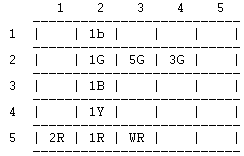
\includegraphics[scale=0.7]{./res/example_2.png}
	\caption{Exemplo de Ambiente Gráfico - preset 1}
	\label{fig:example2}
	\end{center}
	\end{figure}
	
	\begin{figure}[h!]
	\begin{center}
	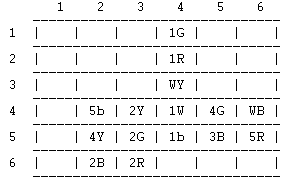
\includegraphics[scale=0.7]{./res/example_3.png}
	\caption{Exemplo de Ambiente Gráfico - preset 2}
	\label{fig:example3}
	\end{center}
	\end{figure}
		
	
	\end{document}
